\documentclass{article}
    % General document formatting
\usepackage[margin=0.7in]{geometry}
\usepackage[parfill]{parskip}
\usepackage[utf8]{inputenc}

% Related to math
\usepackage{amsmath,amssymb,amsfonts,amsthm}
\usepackage{booktabs}
\usepackage{graphicx}

\makeatletter
\def\input@path{ {manuscript/tables/} }
\makeatother

\graphicspath{ {manuscript/figures/} }

\title{Fixed-topology variational methods for relaxed Bayesian phylogenetics}
\author{Christiaan Swanepoel}

\begin{document}

\maketitle
\section*{Introduction}

\section*{Methods}

\section*{Results}

\begin{table}
    \centering
    \begin{tabular}{lrrr}
\toprule
Method &  MCMC &  Variational (mean field) &  Variational (scaled) \\
Statistic        &       &                           &                       \\
\midrule
Pop size         &   96\% &                       89\% &                   87\% \\
Clock rate       &   88\% &                       50\% &                   77\% \\
Rate prior scale &   94\% &                       42\% &                   23\% \\
Node heights     &   94\% &                       76\% &                   84\% \\
Rates            &   94\% &                       79\% &                   92\% \\
Rate mean        &   82\% &                       68\% &                   88\% \\
Rate CoV         &   91\% &                       36\% &                   38\% \\
Tree height      &   91\% &                       60\% &                   66\% \\
Tree length      &   96\% &                       56\% &                   80\% \\
\bottomrule
\end{tabular}

    \caption{Coverage statistics from simulation study}
    \label{tab:coverage}
\end{table}


\begin{figure}
    \centering
    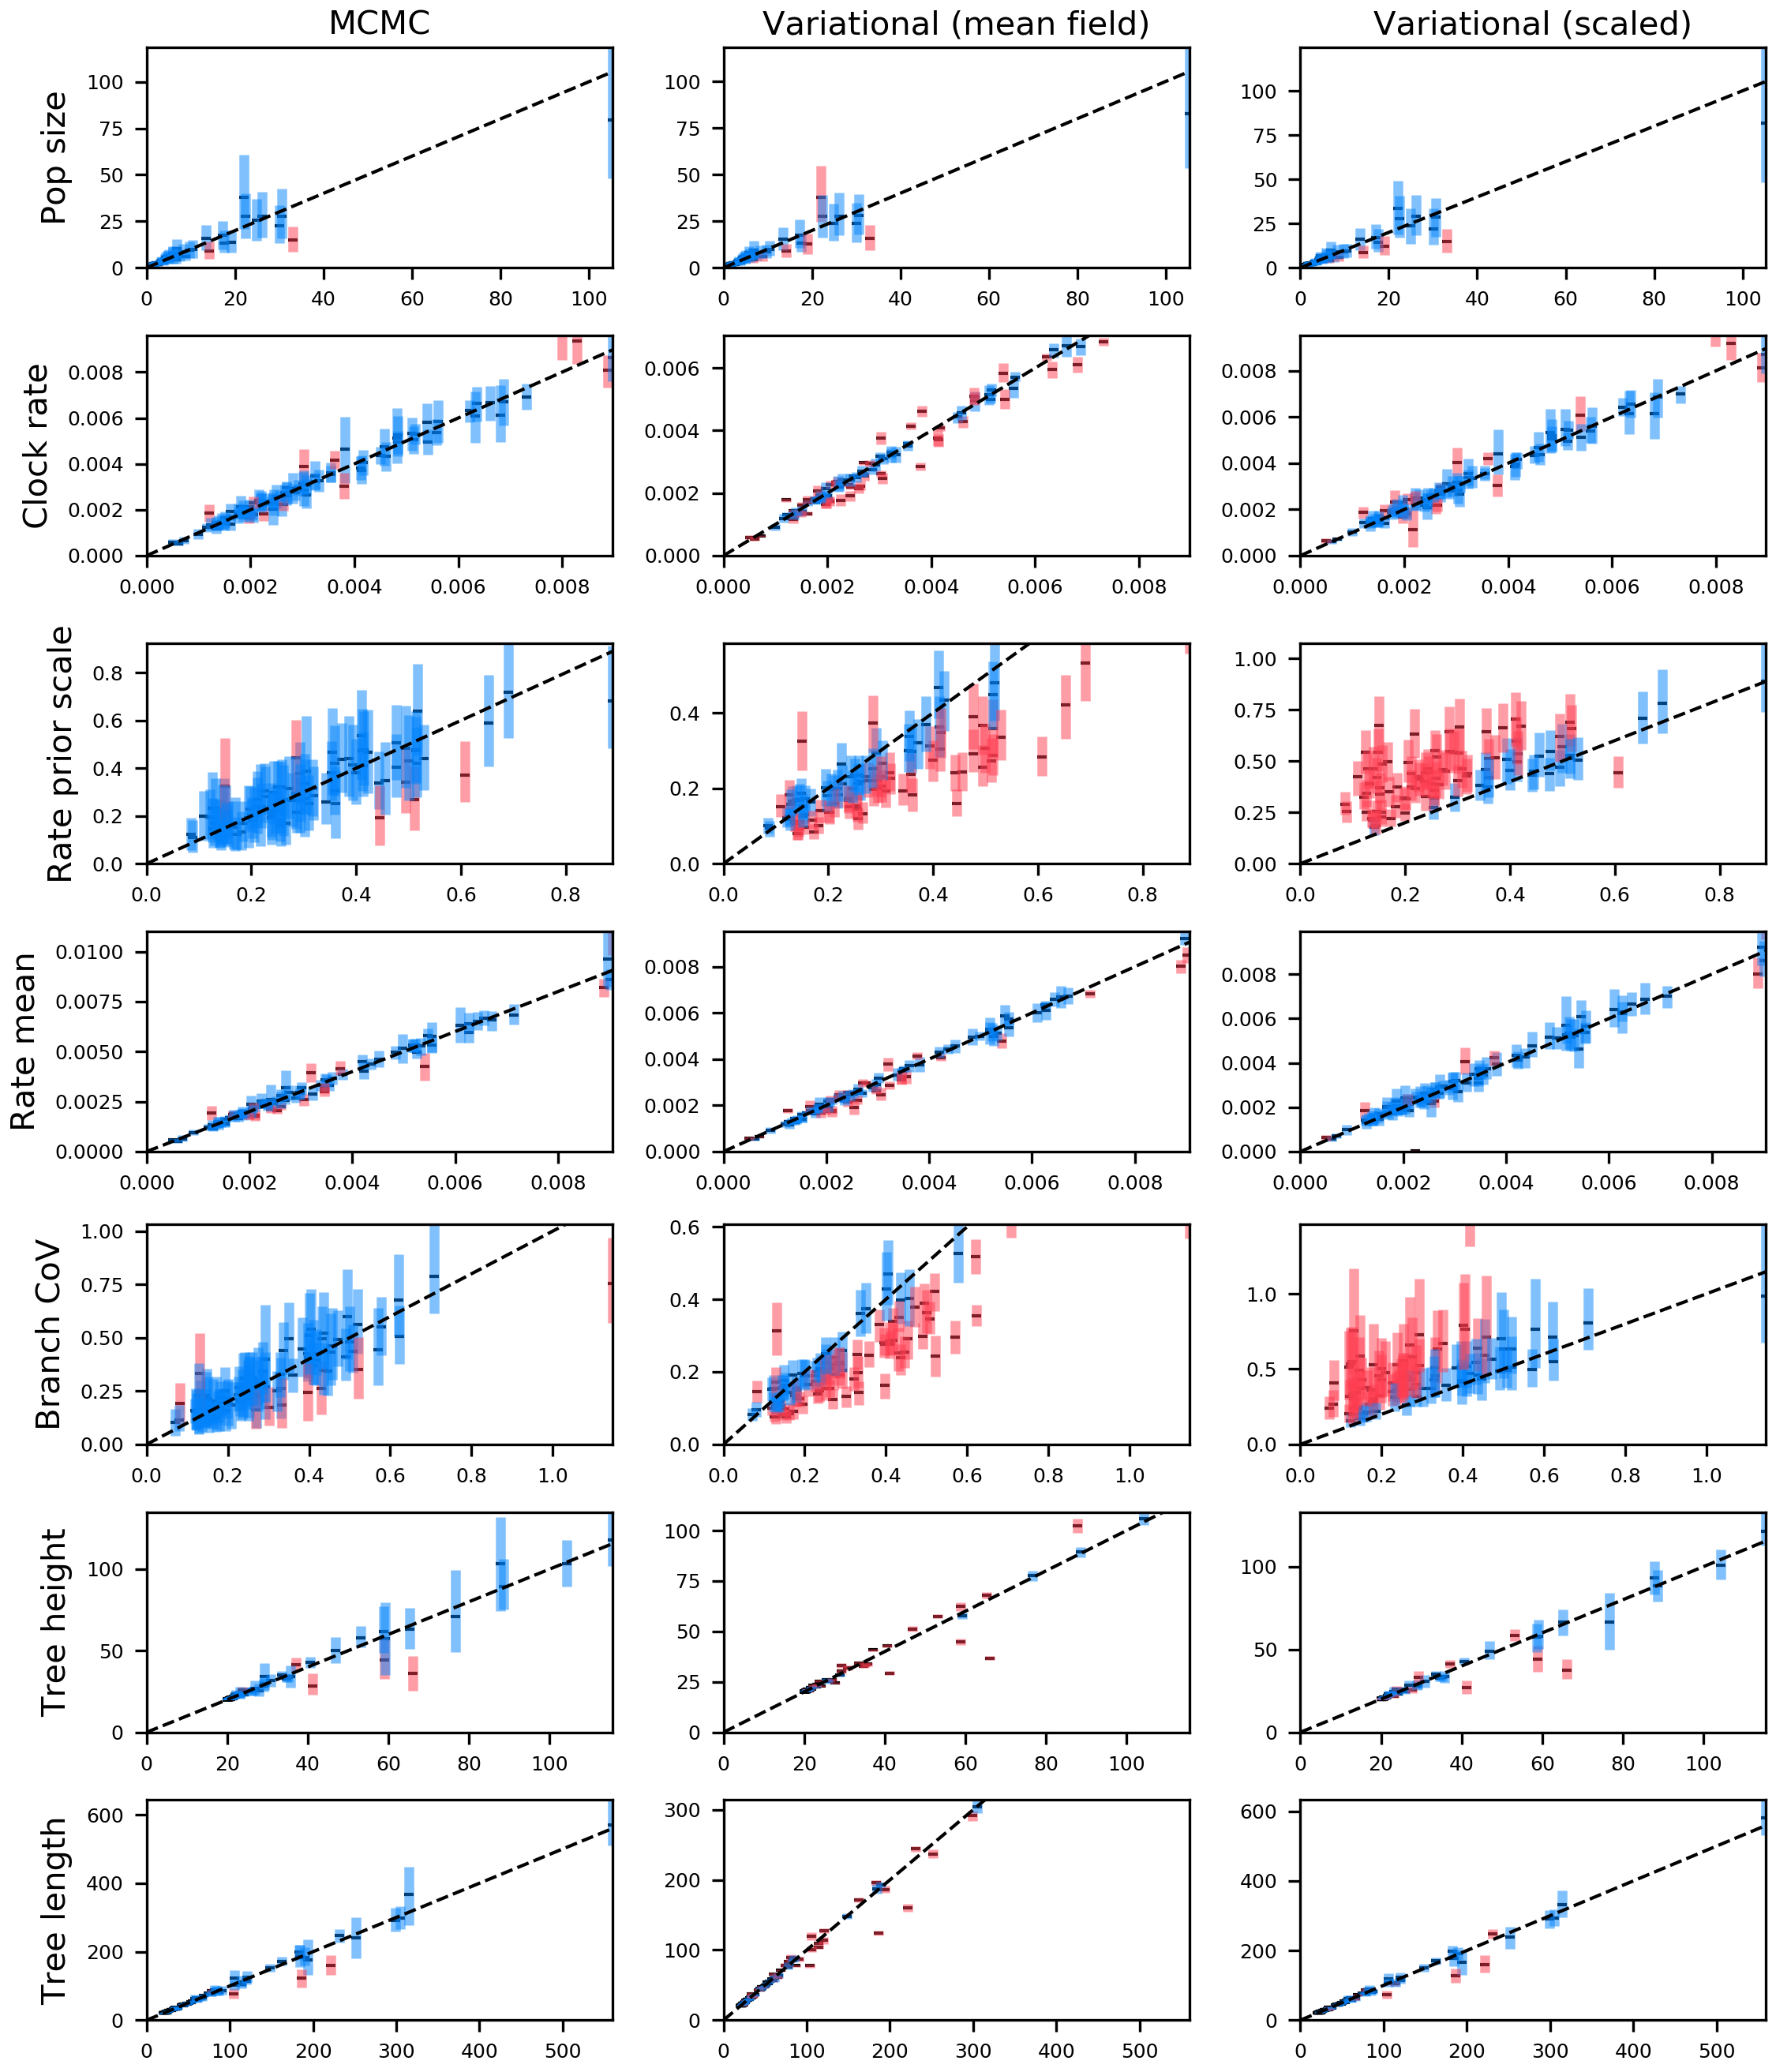
\includegraphics[width=\textwidth]{coverage}
    \caption{Results of simulation study}
    \label{fig:coverage}
\end{figure}
    % Posterior comparison - mean field VS product VS MCMC fixed
% Performance evaluation - Variational vs MCMC - RSV dataset

\section*{Discussion}

\section*{Conclusions}

\end{document}